\documentclass[border=10pt]{standalone}

\usepackage{tikz}
\usepackage{tikzsymbols}
\usetikzlibrary{calc,patterns,shapes.geometric}

\def\centerarc[#1](#2)(#3:#4:#5){\draw[#1] ($(#2)+({#5*cos(#3)},{#5*sin(#3)})$) arc (#3:#4:#5);}

\begin{document}
	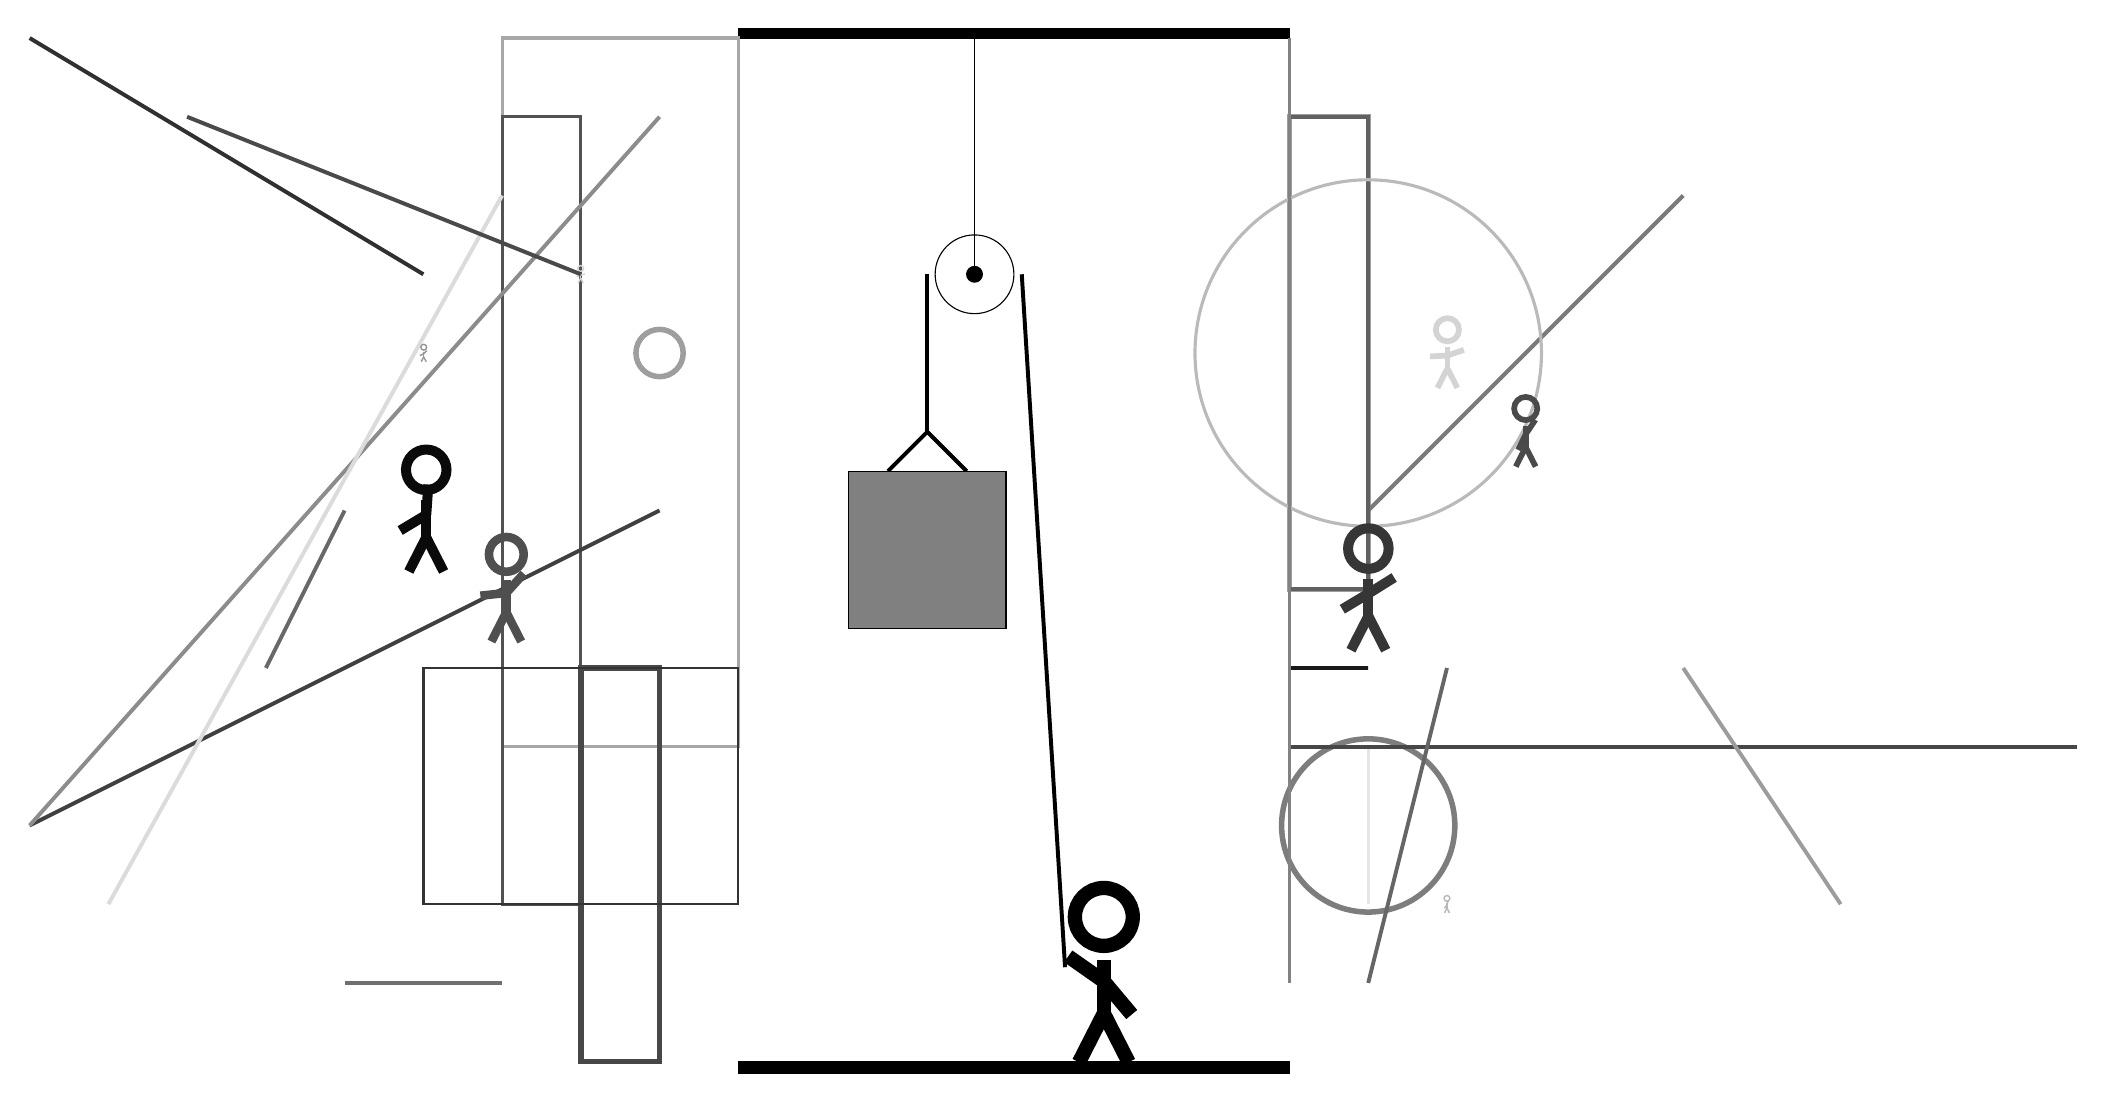
\begin{tikzpicture}
		%%%%% START %%%%%
		
		\draw[fill=black] (-2, 10) rectangle (5, 10.125);
		
		\draw (1, 7) circle (0.5);
		\draw[fill=black] (1, 7) circle (0.1);
		\draw (1, 10) -- (1, 7);
		
		\draw[line width=0.5mm] (-0.1, 4.5) -- (0.4, 5.0) -- (0.9, 4.5);
		\draw[fill=black!50] (-0.6, 4.5) rectangle (1.4, 2.5);
		
		\draw[line width=0.5mm] (0.4, 7) -- (0.4, 5.0);
		\centerarc[line width=0.5mm](1, 7)(0:180:0.6);
		\draw[line width=0.5mm](1.6, 7) -- (2.15, -1.8);
		
		\node[line width=0.4mm, color=black!28] at (7, -1) {\Strichmaxerl[1][52][74]};
		
		\draw[line width=0.6mm, color=black!38] (6, 3) rectangle (5, 9);
		\draw [line width=0.7mm, color=black!38](-3, 6) circle (0.3);
		\draw[line width=0.5mm, color=black!52](10, 8) -- (6, 4);
		\draw[line width=0.4mm, color=black!34] (-2, 10) rectangle (-5, 1);
		\node[line width=0.3mm, color=black!17] at (7, 6) {\Strichmaxerl[4][3][19]};
		\draw[line width=0.4mm, color=black!68] (-4, -1) rectangle (-5, 9);
		\draw[line width=0.5mm, color=black!62] (5, 3) rectangle (6, 9);
		\draw[line width=0.5mm, color=black!81](-6, 7) -- (-11, 10);
		
		\draw[line width=0.5mm, color=black!75](-3, 4) -- (-11, 0);
		\draw[line width=0.7mm, color=black!72] (-4, -3) rectangle (-3, 2);
		\draw[line width=0.5mm, color=black!45](-3, 9) -- (-11, 0);
		\draw[line width=0.3mm, color=black!80] (-2, -1) rectangle (-6, 2);
		\node[line width=0.2mm, color=black!96] at (-6, 4) {\Strichmaxerl[7][31][86]};
		\draw[line width=0.5mm, color=black!56](-5, -2) -- (-7, -2);
		\draw[line width=0.4mm, color=black!90] (6, 2) rectangle (5, 2);
		\draw[line width=0.5mm, color=black!14](-5, 8) -- (-10, -1);
		\node[line width=0.3mm, color=black!17] at (-4, 7) {\Strichmaxerl[1][24][11]};
		\draw [line width=0.4mm, color=black!27](6, 6) circle (2.2);
		\draw [line width=0.7mm, color=black!51](6, 0) circle (1.1);
		\draw[line width=0.4mm, color=black!10] (6, -1) rectangle (6, 1);
		
		\draw[line width=0.5mm, color=black!72](5, 1) -- (15, 1);
		\node[line width=0.5mm, color=black!79] at (6, 3) {\Strichmaxerl[7][31][32]};
		\node[line width=0.7mm, color=black!71] at (8, 5) {\Strichmaxerl[4][64][56]};
		\draw[line width=0.5mm, color=black!39](10, 2) -- (12, -1);
		\node[line width=0.6mm, color=black!41] at (-6, 6) {\Strichmaxerl[1][28][45]};
		\node[line width=0.7mm, color=black!69] at (-5, 3) {\Strichmaxerl[6][6][48]};
		\draw[line width=0.5mm, color=black!59](-7, 4) -- (-8, 2);
		\draw[line width=0.5mm, color=black!60](6, -2) -- (7, 2);
		\draw[line width=0.4mm, color=black!49] (5, -2) rectangle (5, 10);
		\draw[line width=0.5mm, color=black!71](-4, 7) -- (-9, 9);
		
		
		\node at (2.6, -1.9) {\Strichmaxerl[10][-35][-50]};
		
		\draw[fill=black] (-2, -3) rectangle (5, -3.15);
		
		%%%%% END %%%%%
	\end{tikzpicture}
\end{document}